\documentclass{article}
\usepackage{CJKutf8}
\usepackage{multirow}
\usepackage[cmex10]{amsmath}
\usepackage{listings}
\usepackage{algorithmic}
\usepackage{algorithm}
\usepackage{epsfig}
\usepackage{amsopn}
\usepackage{subfigure}
\usepackage{cite}
\usepackage{courier}
\makeatletter
\makeatother
\begin{CJK}{UTF8}{gbsn}
\usepackage[framed,autolinebreaks,useliterate]{mcode}

\usepackage{graphicx}
\begin{document}
\title{通信与网络\\第二次编程作业}
\author{王亭午,2012011018,无210班}
\date{2015年11月18号}
\maketitle
\section{任务一}
某天线接收到的波形为两个实带通信号的迭加,其单边功率谱分别处于10k-11kHz和12k-15kHz,带内为白噪声(假设其分布为零均值的均匀分布),其功率分别为1W和\(10^{-6}\)W。为了对这个接收信号进行可重构采样分析,采样率最低要为多少?\\
答案:根据公式
\begin{equation}
f_s \geq 2(f_H - f_L) (1 + \frac{M}{N})=2(15 - 10) (1 + \frac{0}{N}) = 10\mbox{kHz}
\end{equation}
\section{任务二}
如果采样后先进行均匀量化再存贮,希望保证无量化过载的情况下量化后信噪比达到30dB,最少需要多少位量化? \\
答案:我们先求我们的信号最大最小幅度。
\begin{equation}
P = \int_{-A}^Ap(x)x^2dx = \int_{-A}^A\frac{1}{2A}x^2dx = \frac{A^2}{3} = 1
\end{equation}
得到我们的信号幅度\(A = \sqrt{3}\)。我们考虑到接受信号是白噪声,于是假设\(D = 1\)。
\begin{equation}
\begin{aligned}
SNR & = 10lg\left(\frac{S}{\sigma_q^2}\right)\\
	& = 4.77 + 20lg\left(1\right) + 6.02n \geq 30 \\
\Rightarrow \quad & n \geq 5
\end{aligned}
\end{equation}
\section{任务三}
如果要求最终分离出来的两个实带通信号信噪比均至少达到30dB,需要多少位量化?\\
答案:这个时候我们我们只需把(3)式中S=1换成\(S=10^{-6}\)。这个时候代入(1)得到结果为15。
\section{任务四}
理论计算,并编程仿真,画出原始波形,采样波形,采样频谱,重构波形,重构频谱;采样量化重构后的波形及频谱,重构误差波形及频谱。\\
答案:我们的结果图如下。
(1)可以看到,采样波形根据我们的生产规则,在12-15kHz处值比较大,在10-11kHz处值比较小,其余地方没有值。这是符合我们的期望的。\\
(2)而经过量化之后,频谱各个地方都出现了毛刺,这是我们量化误差导致的频谱上的变化。\\
(3)当我们使用n=5的量化时,12-15kHz的频谱已经可以很好的保证误差在范围内,但是10-11kHz还是没法保证。\\
(3)当我们使用n=15的量化时,所有的频谱已经可以很好的保证误差在范围内。\\
\begin{figure}[!h]
\begin{center}
		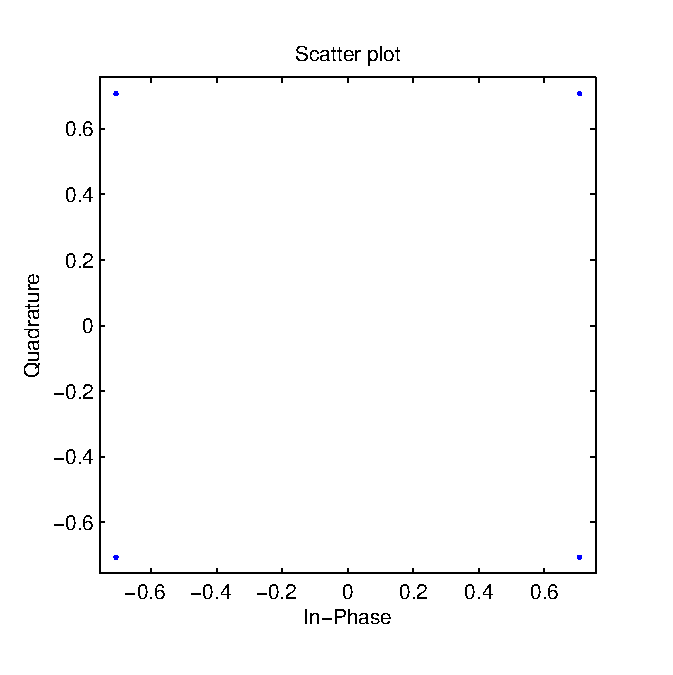
\includegraphics[width=0.8\linewidth]{1.eps}
		\caption{原始波形图}
\end{center}
\end{figure}
\begin{figure}[!h]
\begin{center}
		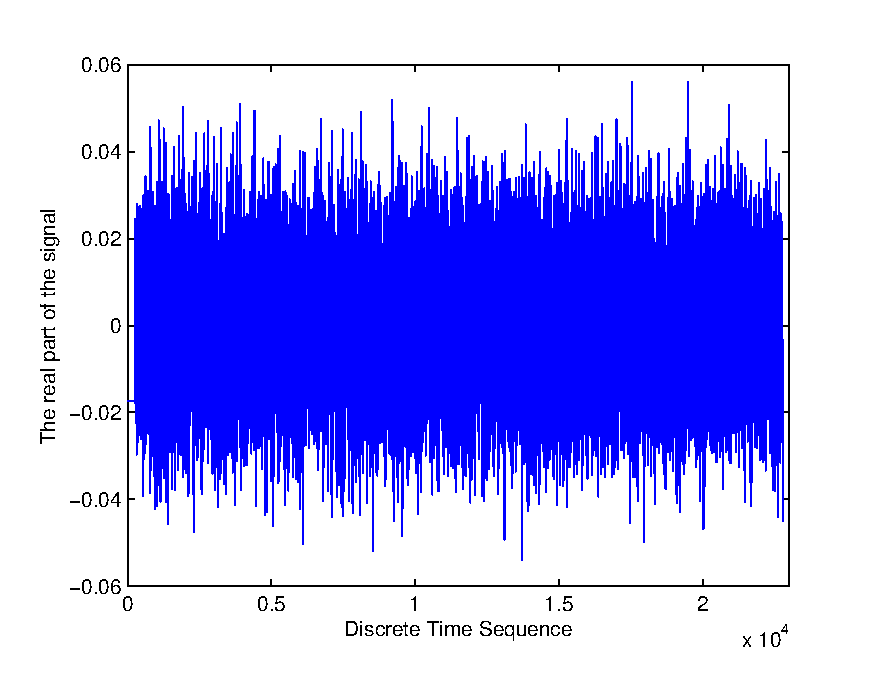
\includegraphics[width=0.8\linewidth]{2.eps}
		\caption{采样波形,采样频谱}
\end{center}
\end{figure}
\begin{figure}[!h]
\begin{center}
		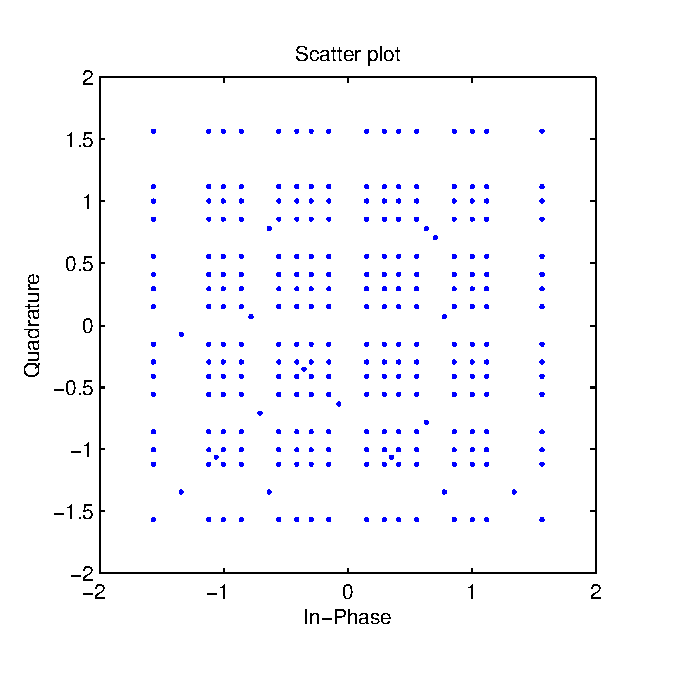
\includegraphics[width=0.8\linewidth]{3.eps}
		\caption{重构波形,重构频谱}
\end{center}
\end{figure}
\begin{figure}[!h]
\begin{center}
		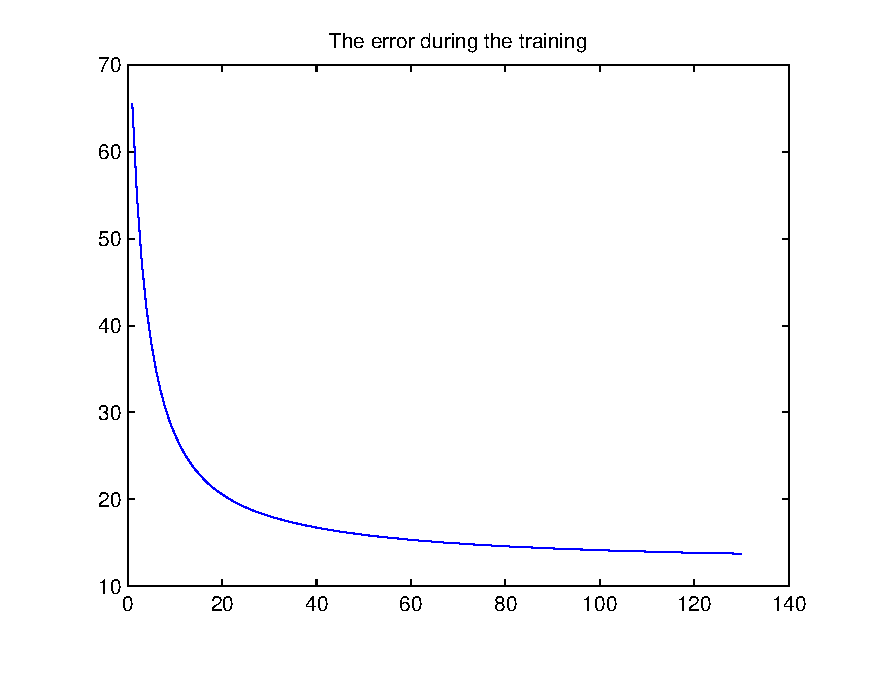
\includegraphics[width=0.8\linewidth]{4.eps}
		\caption{采样量化重构后的波形及频谱}
\end{center}
\end{figure}
\begin{figure}[!h]
\begin{center}
		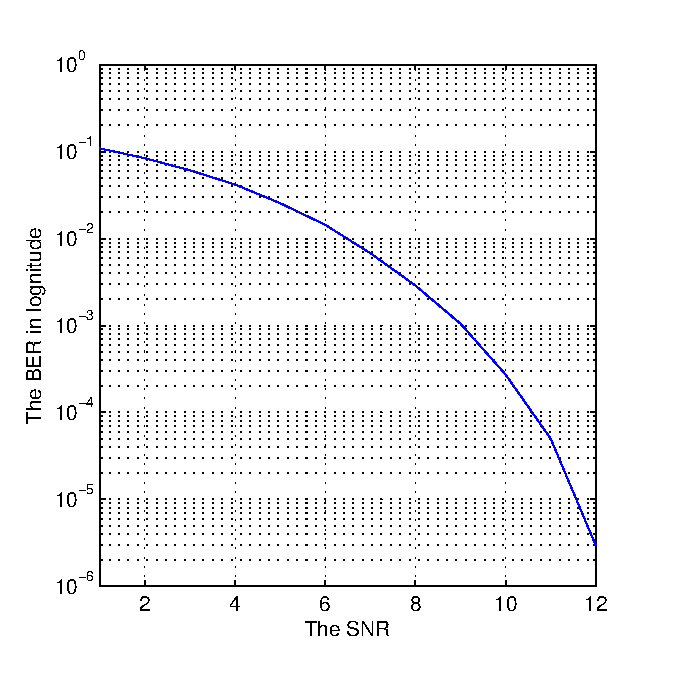
\includegraphics[width=0.8\linewidth]{5.eps}
		\caption{使用n=5重构误差波形及频谱}
\end{center}
\end{figure}
\begin{figure}[!h]
\begin{center}
		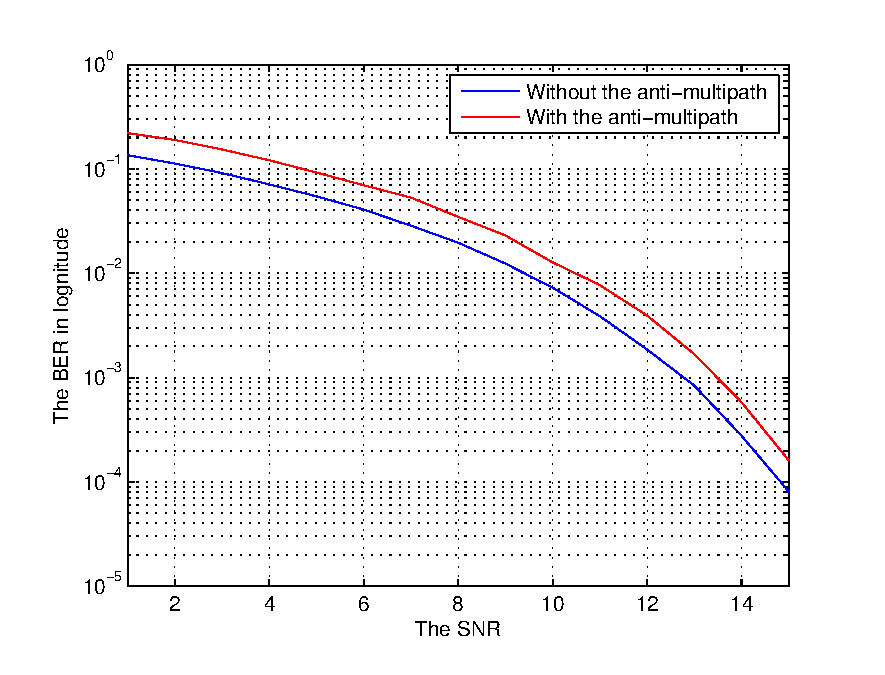
\includegraphics[width=0.8\linewidth]{6.eps}
		\caption{使用n=15重构误差波形及频谱}
\end{center}
\end{figure}

\end{CJK}
\end{document}